%!TEX root = ../terrainbook.tex

\graphicspath{{conversion/}}

\chapter{Conversions between terrain representations}
\label{chap:conversion}

We consider in this chapter the following four terrain representations and discuss the conversions between them:
\vspace{5mm}

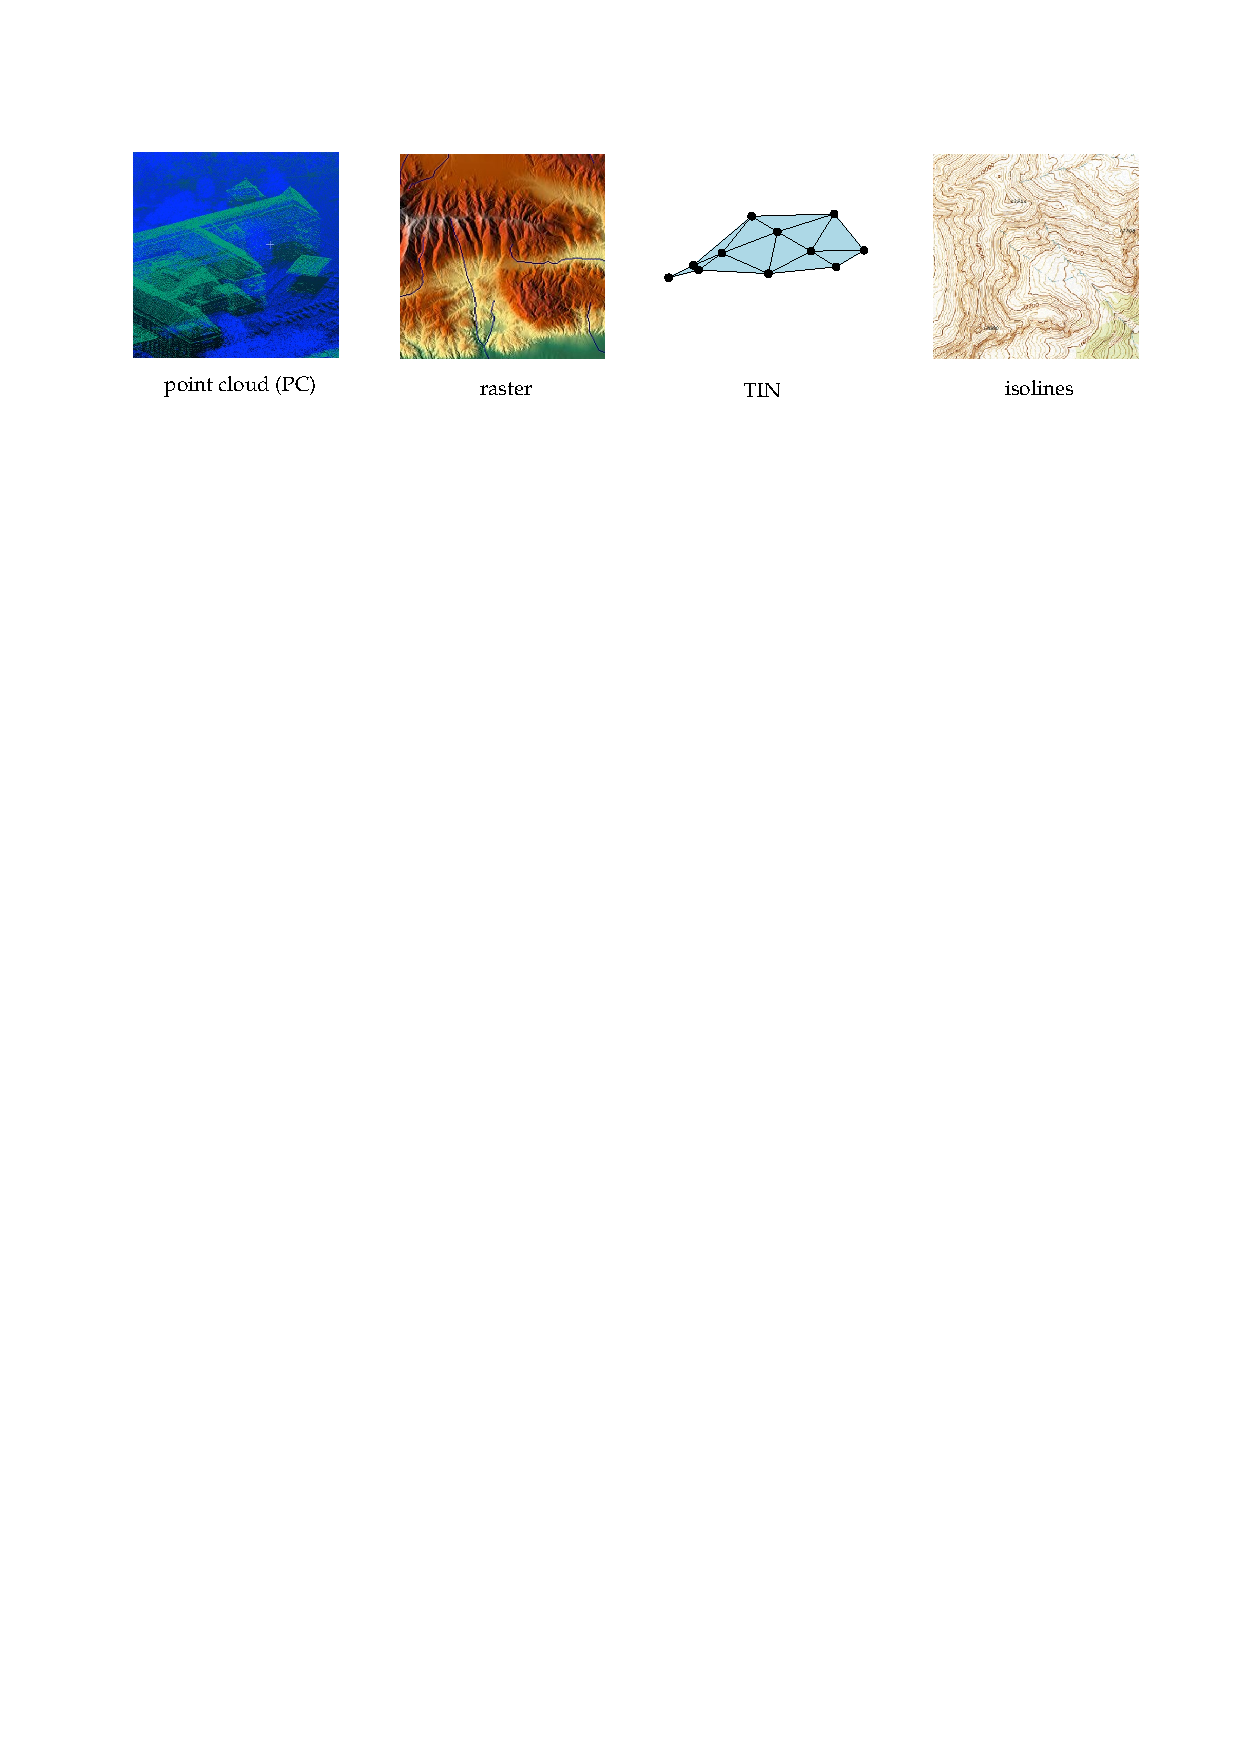
\includegraphics[width=\linewidth]{figs/reps}
\vspace{10mm}

\begin{tabular}{>{\columncolor[gray]{0.9}}l|p{3.0cm}|p{3.0cm}|p{3.0cm}|p{3.0cm}}
\toprule
\rowcolor[gray]{.9}
from/to & PC & raster & TIN & isolines \\ \midrule
PC      & --- & interpolate at middle points of cells (\textsection\ref{sec:r-interpol}) & create DT using 2D projection of points (\ie\ using \(x\) and \(y\) only) & convert to TIN + extract from triangles (\textsection\ref{sec:tin-iso}) + structure output (\textsection\ref{sec:structuring}) \\ \hline
raster  &  keep middle points only & --- & create TIN using middle points of cells + TIN simplification (\textsection\ref{sec:tin-simpl}) & extract from grid cells (\textsection\ref{sec:r-iso}) + structure output (\textsection\ref{sec:structuring}) \\ \hline
TIN     &  keep only vertices & interpolate at middle points of cells (\textsection\ref{sec:r-interpol}) & --- & extract from triangles (\textsection\ref{sec:tin-iso}) + structure output (\textsection\ref{sec:structuring}) \\ \hline
isolines &  keep only vertices --- \emph{warning: `wedding cake' effect} (\textsection\ref{sec:weddingcake}) & convert lines to points + interpolate (\textsection\ref{sec:r-interpol}) --- \emph{warning: `wedding cake' effect} (\textsection\ref{sec:weddingcake}) &  create DT using points --- \emph{warning: `wedding cake' effect} (\textsection\ref{sec:weddingcake}) & --- \\ \bottomrule
\end{tabular}

% \newpage





%%%%%%%%%%%%%%%%%%%%
%
\section{Conversion of PC/TIN to raster}%
\label{sec:r-interpol}

As shown in Figure~\ref{fig:r-interpolation},
\begin{figure}[b]
  \centering
  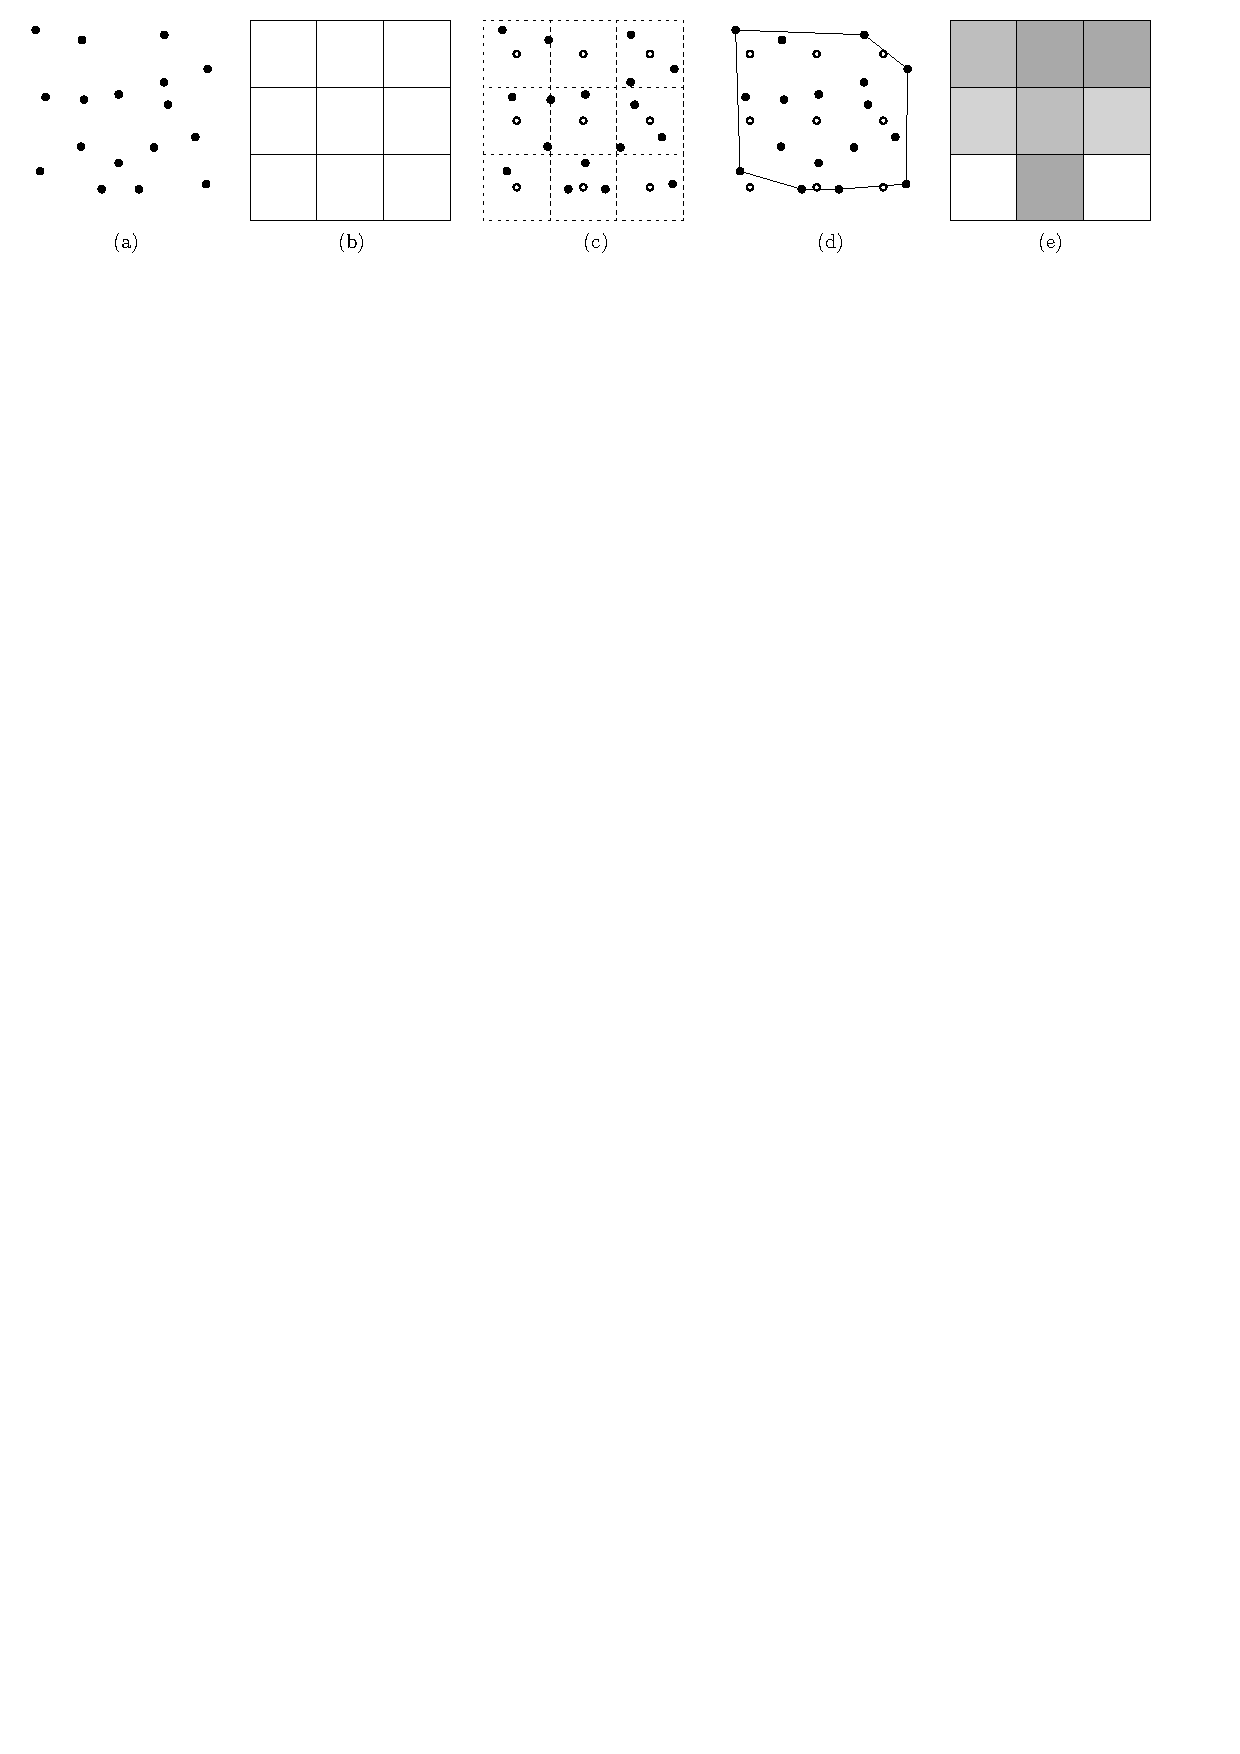
\includegraphics[width=\linewidth]{figs/r-interpolation}
  \caption{\textbf{(a)} input sample points. \textbf{(b)} size/location of output raster. \textbf{(c)} 9 interpolations must be performed (at locations marked with $\circ$): at the middle of each cell. \textbf{(d)} the convex hull of the sample points show that 2 estimations are outside, thus no interpolation. \textbf{(e)} the resulting raster.}%
\label{fig:r-interpolation}
\end{figure}
this step is trivial: one needs to interpolate at the locations of the centre points of the raster cells.
The interpolation method can be any of the ones described in Chapters~\ref{chap:interpol} and~\ref{chap:kriging}.






%%%%%%%%%%%%%%%%%%%%
%
\section{Conversion to isolines}%
\label{sec:iso}

Reading a contour map requires some skill, however it is considerably easier to learn to interpret a contour map than to manually draw one from a limited set of sample points.
Yet this was exactly the task of many cartographers in the past couple of centuries: it was intuitively done by imagining a local triangulation of sample points. 
% As is the case with many cartographic skills, the skill is developed through practice and experience. 
% Consequently, the exact thought process behind the skill is difficult to capture in a fixed algorithm. 

%

Isolines are usually directly extracted from either a TIN or a grid representation of a terrain. 
The basic idea, as shown in Figure~\ref{fig:isolineidea},
\begin{figure}
  \centering
  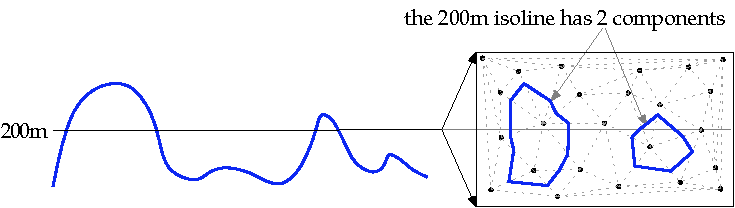
\includegraphics[width=0.9\textwidth]{figs/isoline}
  \caption{Vertical cross-section of a terrain (left), and a 2D projection of the terrain TIN with the extracted 200m isoline (right).}%
\label{fig:isolineidea}
\end{figure}
is to compute the intersection between a level value (\eg\ 200m) and each cell of the terrain (triangle or grid cell in our case).
Notice that the cells are `lifted' to their elevation.  
Each cell of the terrain is thus visited, one after the other, and for each cell if there is an intersection (which forms a line segment) then it is extracted.
The resulting set of segment lines forms an approximation of the isoline.
This process is then repeated for every level value.
Notice that an isoline can have several \emph{components}, for instance when the terrain has more than one peak.

Therefore the number and size of the line segments in the resulting isoline are dependent on the resolution of the data representation. 
% Consequently by refining that data representation, \eg\ by performing interpolation, the resolution of the contour lines is improved.

%

The basic algorithm for extracting one isoline is shown in Algorithm~\ref{algo:iso}.
\begin{algorithm}[tb] 
  \KwIn{a planar partition $E$ formed of cells (either rectangular or triangular cells); the elevation value $z_0$}
  \KwOut{a list of unstructured line segments representing the contour lines at $z_0$}
  $segmentList \leftarrow [\;]$ \;
  \For{$e \in E$}
  {
    \If{$z_0$ intersects $e$} 
    {
      \tcc{See Figures~\ref{fig:rasterconfs} and~\ref{fig:isoline-tr}} 
      extract intersection $\chi$ of $z_0$ with $e$\;
      add $\chi$ to $segmentList$\;
    }
  }
  \caption{Simple extraction of one isoline}
\label{algo:iso}
\end{algorithm} 
\begin{figure}
  \centering
  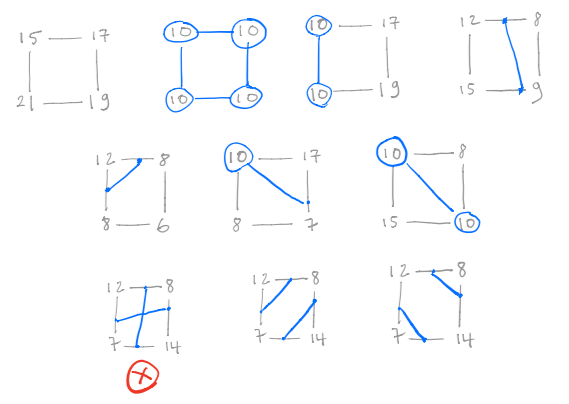
\includegraphics[width=0.95\linewidth]{figs/isoline-square}
\caption{Different cases when extracting an isoline at elevation 10m for a regular grid. The grey values are the elevation of the vertices forming one regular cell, and the blue lines and vertices are the ones extracted for that cell.}
\label{fig:rasterconfs}
\end{figure}
\begin{figure}
  \centering
  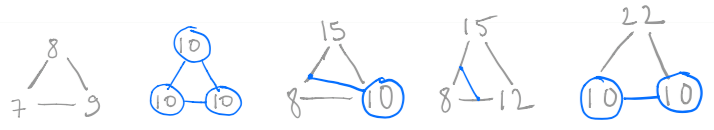
\includegraphics[width=0.95\linewidth]{figs/isoline-tr}
\caption{Different cases when extracting an isoline at elevation 10m for a TIN. The grey values are the elevation of the vertices forming one triangle, and the blue lines and vertices are the ones extracted for that triangle.}
\label{fig:isoline-tr}
\end{figure}
Note that since the algorithm contours every grid cell or triangle individually and requires only local information, it is very easy to parallelise. 
It is thus a scalable algorithm.
Its time complexity is $\mathcal{O}(c)$, where $c$ is the number of cells.
Recall from Chapter~\ref{chap:dtvd} that for $n$ points a DT contains about $2n$ triangles.

The same idea can be used to extract all the isolines: for each triangle/cell and each level value, extract all the necessary line segments.


%%%
\subsection{Conversion of raster to isolines}%
\label{sec:r-iso}

% In the case of contouring a raster  the dotted lines in Figure~\ref{fig:rastercontscheme}. 
Intersections are computed by linearly interpolating the elevations of the vertex pairs along the edges of this grid.
Figure~\ref{fig:rasterconfs} illustrates the different possible configurations. 
The top-left case indicates the case for which there are no intersections: all vertices are either higher or lower than $z_0$. 

Observe that two vertices are exactly at $z_0$, then the extraction of these is in theory not necessary because the neighbouring cell could also extract them. 
However, we do not want to obtain an output with duplicate line segments, and thus a simple solution to this is to only extract such line segments if they are for instance the lower and/or left segments of a given cell.

The most interesting case is the bottom-left one in Figure~\ref{fig:rasterconfs}, it occurs when the two pairs of opposing points are respectively higher and lower than $z_0$.
This forms a saddle point. 
The ambiguity arises here since there are two ways to extract a valid pair of contour line segments (only one of the 2 options must be extracted).
This can be resolved by simply picking a random option or consistently choose one geometric orientation. 


%%%
\subsection{Conversion TIN to isolines}
\label{sec:tin-iso}

Since a triangle has one fewer vertex/edge than a square grid cell, there are less possible intersection cases (Figure~\ref{fig:isoline-tr}) and, more importantly, there is no ambiguous case. 
The worst case to handle is when there are horizontal triangles at exactly the height of the isoline.
Otherwise, the intersection cases are quite similar to the raster situation and they can be easily implemented.

To avoid extracting twice the same line segment when 2 vertices are at $z_0$ (case on the right in Figure~\ref{fig:isoline-tr}), then we can simply look at the normal of the edge segment: if its $y$-component is positive then it can be added, if $y=0$ then only add if the $x$-component is positive.

Observe that since the algorithm is simpler than that for a raster dataset, one way to extract isolines from a raster dataset is by first triangulating it: each square cell is subdivided into 2 triangles (simply ensure that the diagonal is consistent, \eg\ from lower-left to top-right).


% TODO : interval tree?

% % It is possible to define an additional data structure, called the \emph{interval tree}, that helps us for the fast localization of triangles that intersect a certain height. 
% % The method delivers connected isolines, so no line merging needs to be performed as with \Call{GenerateContours}{}. \citet{van1997contour} also propose a somewhat similar approach that is based on the slightly more sophisticated \emph{contour tree} (also known as the \emph{Reeb graph}).


% % \citet{van1994efficient} proposes a more efficient algorithm to compute contours for a \ac{tin}. It requires an additional data structure, the \emph{interval tree}, that aids fast localization of triangles that intersect a certain depth. Compared to the brute-force \Call{GenerateContours}{}, this approach has two advantages. Firstly, not all triangles need to be visited during contouring, which is especially beneficial when the requested contour line does not intersect a large portion of the triangles. And secondly, the method delivers connected contour segments straight away, so no line merging needs to be performed as with \Call{GenerateContours}{}. \citet{van1997contour} also propose a somewhat similar approach that is based on the slightly more sophisticated \emph{contour tree} (also known as the \emph{Reeb graph}).

% % Given that the auxiliary data structure is available, these approaches can compute a set of contour lines in logarithmic time, compared to linear time for \Call{GenerateContours}{}.


%%%
\subsection{Structuring the output}%
\label{sec:structuring}

The line segments obtained from the simple algorithms above are not structured, \ie\ they are in an arbitrary order (the order in which we visited the triangles/cells) and are not connected.
Furthermore, the set of line segments can form more than one \emph{component}, a set of segments forming a closed polygon (unless they are at the border of the dataset).
Perhaps the only application where having unstructured line segments is fine is for visualisation of the lines.
For most other applications this can be problematic, for instance:
\begin{enumerate}
  \item if one wants to know how many peaks above 1000m there are in a given area;
  \item if smoothing of the isolines is necessary, with the Douglas-Peucker algorithm for instance;
  \item if a GIS format requires that the isolines be closed polylines oriented such that the higher terrain is on the left for instance, such as for colouring the area enclosed by an isoline.
\end{enumerate}

%

To obtain structured segments, the simplest solution is to merge, as post-processing, the line segments based on their start and end vertices.
Observe that the line segments will not be consistently oriented to form one polygon (see Figure~\ref{fig:isoline2}a), that is the orientation of the segments might need to be swapped.
This can be done by simply starting with a segment $ab$, and searching for the other segment having $b$ as either start or end vertex, and continue until a component is formed (a polygon is formed), or until no segment can be found (the border of the dataset is reached, as shown in Figure~\ref{fig:isoline2}a).
\begin{figure}
  \centering
  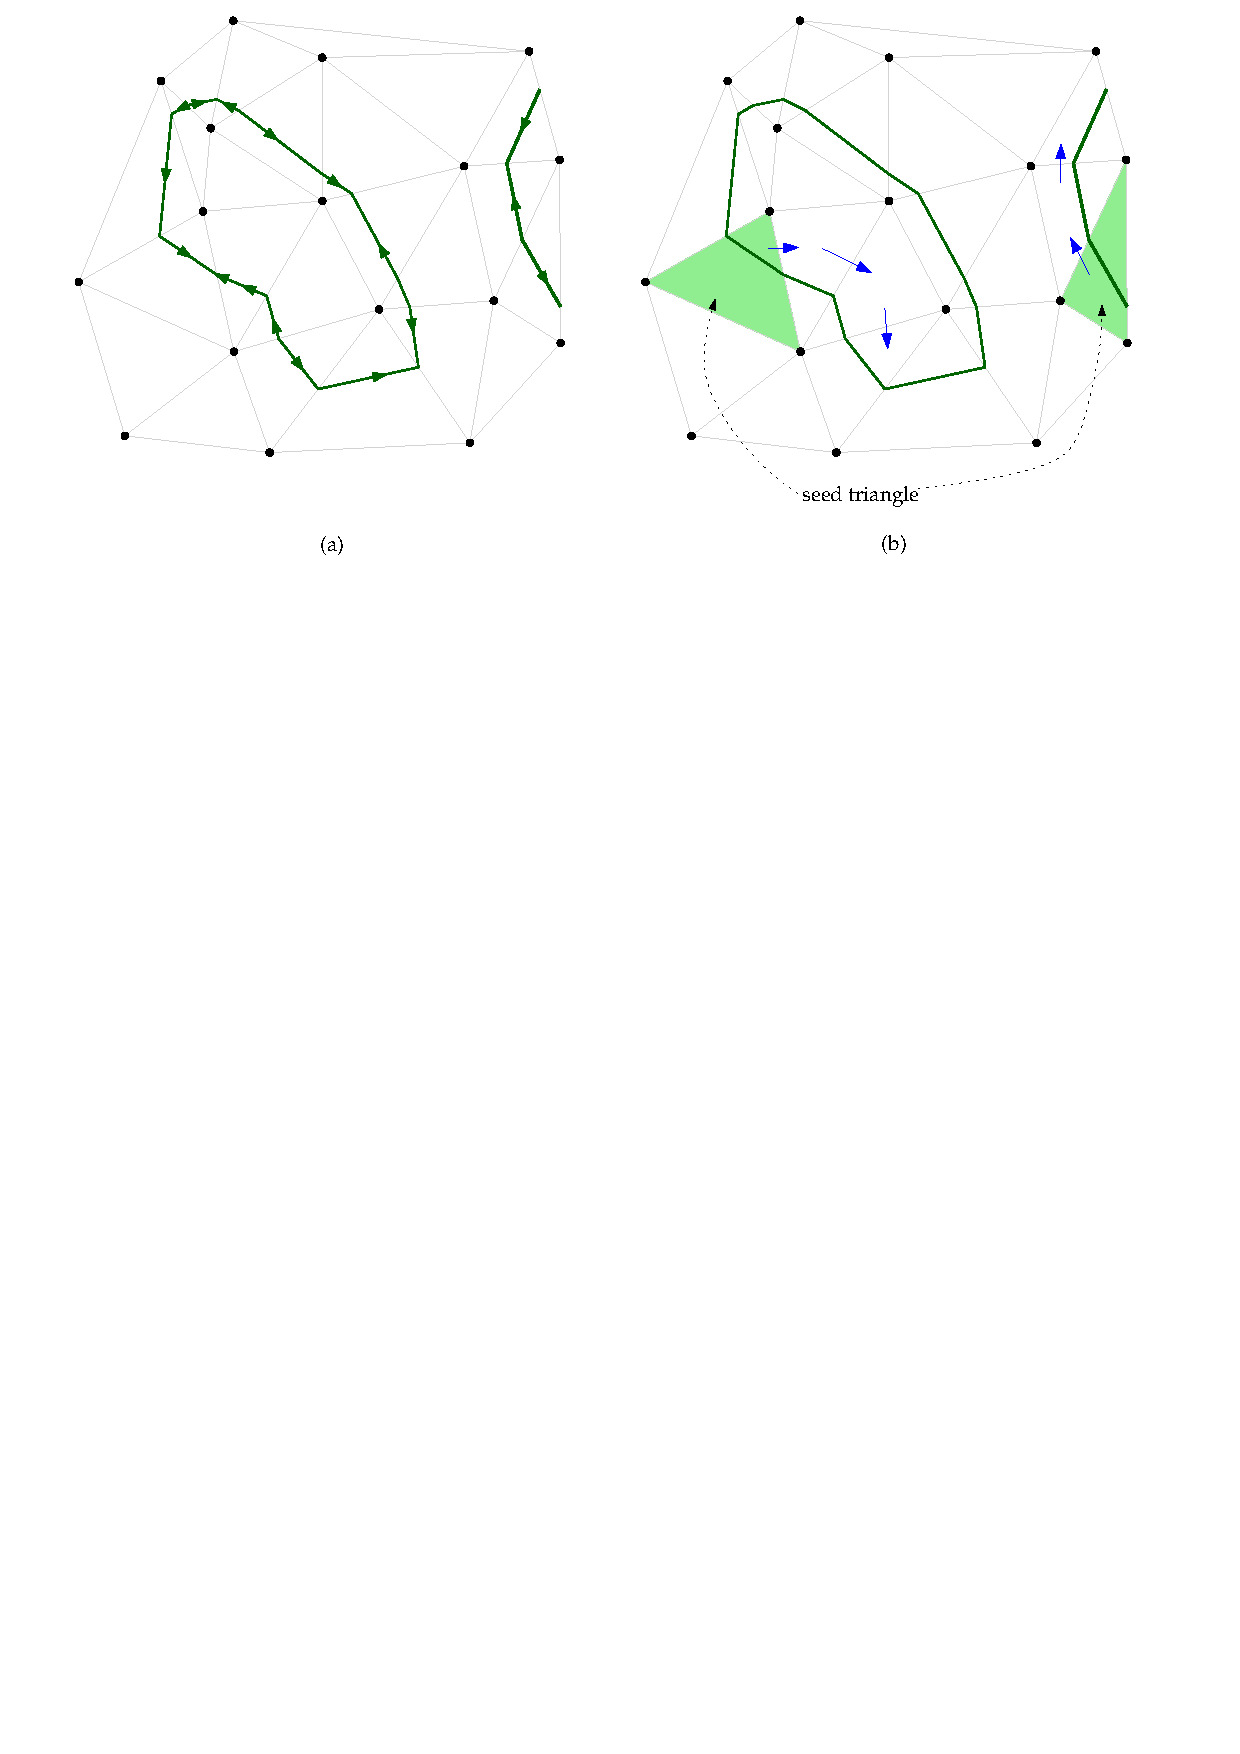
\includegraphics[width=\linewidth]{figs/isoline2}
  \caption{\textbf{(a)} The isoline segments extracted with Algorithm~\ref{algo:iso} do not have a consistent orientation. \textbf{(b)} Algorithm~\ref{algo:iso} can be sped up by starting at a seed triangle and `tracing' the isoline; the order is shown by the blue arrows.}%
\label{fig:isoline2}
\end{figure}

%

As shown in Figure~\ref{fig:isoline2}b, another solution is to find \emph{one} cell $\tau_0$ intersecting the isoline at a given elevation, `tracing' the isoline by navigating from $\tau_0$ to the adjacent cell, and continuing until $\tau_0$ is visited again (or the border of the dataset is reached).
To navigate to the adjacent cell, it suffices to identify the edge $\epsilon$ intersecting the isoline, and then navigating to the triangle/cell that is incident to $\epsilon$.
It is possible that there is no adjacent cell, if the boundary of the convex hull is reached in a TIN for instance.
This requires that the TIN be stored in a topological data structure in which the adjacency between the triangles is available (for a grid this is implied).

The main issue is finding the starting cells (let us call them seed triangles).
Obviously, it suffices to have one seed for each of the component of the isolines (there would be 2 seeds in Figure~\ref{fig:isoline2}b).
An easy algorithm to extract all the components of an isoline requires visiting all the cells in a terrain, and keeping track of which triangles have been visited (simply store an Boolean attribute for each triangle, which is called a \emph{mark bit}).
Simply visit triangle sequentially and mark them as `visited', when one triangle has an intersection then start the tracing operation, marking triangles as visited as you trace. 


%%%
\subsection{Smoothness of the contours}
\label{sec:smoothness-contours}

The mathematical concept of the \emph{Implicit Function Theorem} states that a contour line extracted from a field $f$ will be no less smooth than $f$ itself.
In other words, obtaining smooth contour lines can be achieved by smoothing the field itself.
Robin Sibson\footnote{http://citeseerx.ist.psu.edu/viewdoc/summary?doi=10.1.1.51.63} goes further in stating that:
\begin{quote}
  \emph{`The eye is very good at detecting gaps and corners, but very bad at detecting discontinuities in derivatives higher than the first. 
  For contour lines to be accepted by the eye as a description of a function however smooth, they need to have continuously turning tangents, but higher order continuity of the supposed contours is not needed for them to be visually convincing.'}
\end{quote}
In brief, in practice we should use interpolant functions whose first derivative is continuous (\ie\ C$^1$) if we want to obtain smooth contours. 
C$^0$ interpolants are not enough, and C$^2$ ones are not necessary.


%%%%%%%%%%%%%%%%%%%%
%
\section{Simplification of a TIN}
\label{sec:tin-simpl}

The TIN simplification problem is:
\begin{quote}
	Given a TIN formed by the Delaunay triangulation of a set $S$ of points, the aim is to find a subset $R$ of $S$ which will approximate the surface of the TIN as accurately as possible, using as few points as possible. The subset $R$ will contain the `important' points of $S$, \ie\ a point $p$ is important when the elevation at location $p$ can not be accurately estimated by using the neighbours of $p$.
\end{quote}

The overarching goal of TIN simplification is always to (smartly) reduce the number of points in the TIN\@.
This reduces memory and storage requirements, and speeds up TIN analysis algorithms.

Observe that the simplification of a TIN can be used to simplify a raster terrain: we can first obtain the triangulation of the middle points of each cell, and then simplify this TIN to obtain a simplified terrain.


\subsection{The importance of a point}
The importance of a point is a measure that indicates the error in the TIN when that point would not be part of it. 
Imagine for instance a large flat area in a terrain. 
This area can be accurately approximated with only a few large triangles, and inserting points in the middle of such an area does not make the TIN more accurate. 
An area with a lot of relief on the other hand can only be accurately modelled with many small triangles. 
We can therefore say that the points in the middle of the flat area are less important than the points in the area with relief.

The importance of a point---or importance measure---can be expressed in several ways, \eg\  based on an elevation difference or the curvature of the point. Here we focus on the \emph{vertical error} which has proven to be effective in practice.

The vertical error of a point $p$ is the elevation difference between $p$ itself and the interpolated elevation in the TIN $\mathcal{T}$ at the $(x,y)$ coordinates of $p$ (see Figure~\ref{fig:meshsimplification}).  
Notice that $\mathcal{T}$ does not contain $p$ as a vertex.

\begin{figure}
	\centering
	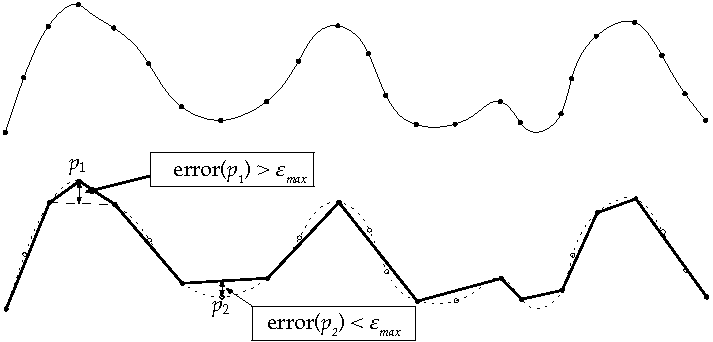
\includegraphics[width=0.85\linewidth]{figs/mesh_simplification}
	\caption{The importance measure of a point can be expressed by its vertical error. When this error is greater than a given threshold $\epsilon_{max}$, the point is kept ($p_1$), else it is discarded ($p_2$).}
	\label{fig:meshsimplification}
\end{figure}


\subsection{TIN simplification algorithms}

There are two main approaches to TIN simplification: decimation and refinement. 
In a decimation algorithm, we start with a TIN that contains all the input points, and gradually remove points that are not important. 
In a refinement algorithm, we do the opposite: we start with a very simple TIN, and we gradually refine it by adding the important points. 


\subsubsection{TIN simplification by refinement}
Here we describe an iterative refinement algorithm based on greedy insertion\footnote{A greedy algorithm is one that divides a complex problem into a series of easier steps, then solves it by making the locally optimal choice at each step, and never goes back on this choice.
In our case the heuristic is the importance measure, \ie\ the vertical error. See \url{https://en.wikipedia.org/wiki/Greedy_algorithm}.}. 
It begins with a simple triangulation of the spatial extent and, at each iteration, finds the input point with highest importance---the highest vertical error---in the current TIN and inserts it as a new vertex in the triangulation. 
The algorithm stops when the highest error of the remaining input points with respect to the current TIN is below a user-defined threshold $\epsilon_{max}$. Algorithm~\ref{algo:tin-simp:ref} shows the pseudo-code.
It is also possible to insert only a certain percentage of the number of input points, \eg\ we might want to keep only 10\% of them.

\begin{algorithm}[tb] 
	\KwIn{A set of input points $S$, and the simplification threshold $\epsilon_{max}$}
	\KwOut{A triangulation $\mathcal{T}$ that consists of a subset of $S$ and that satisfies $\epsilon_{max}$}
	Construct an initial triangulation $\mathcal{T}$ that covers the 2D bounding box of $S$ \;
	$\epsilon \leftarrow \infty$ \;
	% \tcc{keep iterating as long as the maximum vertical error $\epsilon$ is greater than our threshold $\epsilon_{max}$:}
	\While{$\epsilon > \epsilon_{max}$}
	{
		% \tcc{recompute all errors and find the current maximum error $\epsilon$ and the corresponding point $q$:}
		$\epsilon \leftarrow$ 0 \;
		$q \leftarrow$ nil \;
		\For{all $p \in S$} 
		{
			$\tau \leftarrow$ the triangle in $\mathcal{T}$ that contains $p$ \;
			$\epsilon_{\tau} \leftarrow$ the vertical error of $p$ with respect to $\tau$ \;
			\If{$\epsilon_{\tau} > \epsilon$}{
				$\epsilon \leftarrow \epsilon_{\tau}$ \;
				$q \leftarrow p$ \;
			}
		}
		\tcc{insert the point $q$ that has the largest error:}
		insert into $\mathcal{T}$ the point $q$ \;
		remove $q$ from $S$ \;
	}
	\caption{TIN simplification by refinement}
	\label{algo:tin-simp:ref}
\end{algorithm}

\subsubsection{TIN simplification by decimation}
The implementation of the decimation algorithm is similar to the refinement algorithm. The main differences are 
\begin{enumerate}
	\item we start with a full triangulation of all the input points, instead of an empty triangulation;
	\item instead of iteratively adding the point with the highest importance, we iteratively remove the point with the lowest importance, and
	\item in order to compute the importance of a point we actually need to remove it \emph{temporarily} from the triangulation before we can decide if it should be permanently removed. In other words: we need to verify what the vertical error would be if the point was not present. 
\end{enumerate}

Algorithm~\ref{algo:tin-simp:dec} shows the pseudo-code for the TIN decimation algorithm.
\begin{algorithm}[tb] 
	\KwIn{A set of input points $S$, and the simplification threshold $\epsilon_{max}$}
	\KwOut{A triangulation $\mathcal{T}$ that consists of a subset of $S$ and satisfies $\epsilon_{max}$}
	$\mathcal{T} \leftarrow$ a triangulation of $S$ \;
	$\epsilon \leftarrow 0$ \;
	% \tcc{keep iterating as long as the maximum vertical error $\epsilon$ is smaller than our threshold $\epsilon_{max}$:}
	\While{$\epsilon < \epsilon_{max}$}
	{
		% \tcc{recompute all errors and find the current minimum error $\epsilon$ and the corresponding point $q$:}
		$\epsilon \leftarrow \infty$  \;
		$q \leftarrow$ nil \;
		\For{all $p \in \mathcal{T}$}
		{
			remove $p$ from $\mathcal{T}$ \;
			$\tau \leftarrow$ the triangle in $\mathcal{T}$ that contains $p$ \;
			$\epsilon_{\tau} \leftarrow$ the vertical error of $p$ with respect to $\tau$ \;
			\If{$\epsilon_{\tau} < \epsilon$}{
				$\epsilon \leftarrow \epsilon_{\tau}$ \;
				$q \leftarrow p$ \;
			}
			put back $p$ into $\mathcal{T}$ \;
		}
		\tcc{remove the point $q$ that has the smallest error:}
		remove from $\mathcal{T}$ the point $q$ \;
	}
	\caption{TIN simplification by decimation}
	\label{algo:tin-simp:dec}
\end{algorithm}
It should be noticed that the implementation of this algorithm requires a method to delete/remove a vertex from a (Delaunay) triangulation, and that many libraries do not have one\footnote{The implementation in SciPy does not allow to remove one vertex, but CGAL does (\url{www.cgal.org})}.

Observe that the Algorithms~\ref{algo:tin-simp:ref} and~\ref{algo:tin-simp:dec} both state that the importance of the points must be completely recomputed after each iteration of the algorithms (either one removal or one insertion), but that in practice several of these will not have changed.
As can be seen in \refchap{chap:dtvd}, the insertion/deletion of a single point/vertex will only \emph{locally} modify the triangulation, and it is thus faster from a computational point of view to flag the vertices incident to the modified triangles, and only update these.


%%%
%
\subsection{Comparison: decimation versus refinement}

%

While both methods will allow us to obtain similar results, the properties of the resulting terrain are different.
Consider the threshold $\epsilon_{max}$ that is used to stop the simplification process.
If the refinement method is used, then it is guaranteed that the final surface of the terrain will be at a maximum of $\epsilon_{max}$ (vertical distance) to the `real surface' because all the points of the input are considered.
However, with the decimation method, after a vertex is deleted from the TIN, it is never considered again when assessing whether a given vertex has an error larger than $\epsilon_{max}$. 
It is thus possible that the final surface does not lie within $\epsilon_{max}$, although for normal distribution of points, it should not deviate too much from it.

%

In practice, refinement is often computationally more efficient than decimation because we do not need to first build a TIN from all input points before removing several of them again. 
However, decimation could be more efficient when you already have a detailed TIN, stored in a topological data structure, that just needs to be slightly simplified.

%%%%%%%%%%%%%%%%%%%%
%
\section{Conversion isolines to TIN/raster creates the `wedding cake effect'}%
\label{sec:weddingcake}

If the input is a set of isolines, then the simplest solution is, as shown in Figure~\ref{fig:wedding}a, to convert these to points and then use any of the interpolation methods previously discussed.
This conversion can be done by either keeping only the vertices of the polylines, or by sampling points at regular intervals along the lines (say every 10m).
\begin{figure}
  \centering
  \begin{subfigure}[b]{0.2\linewidth}
    \centering
    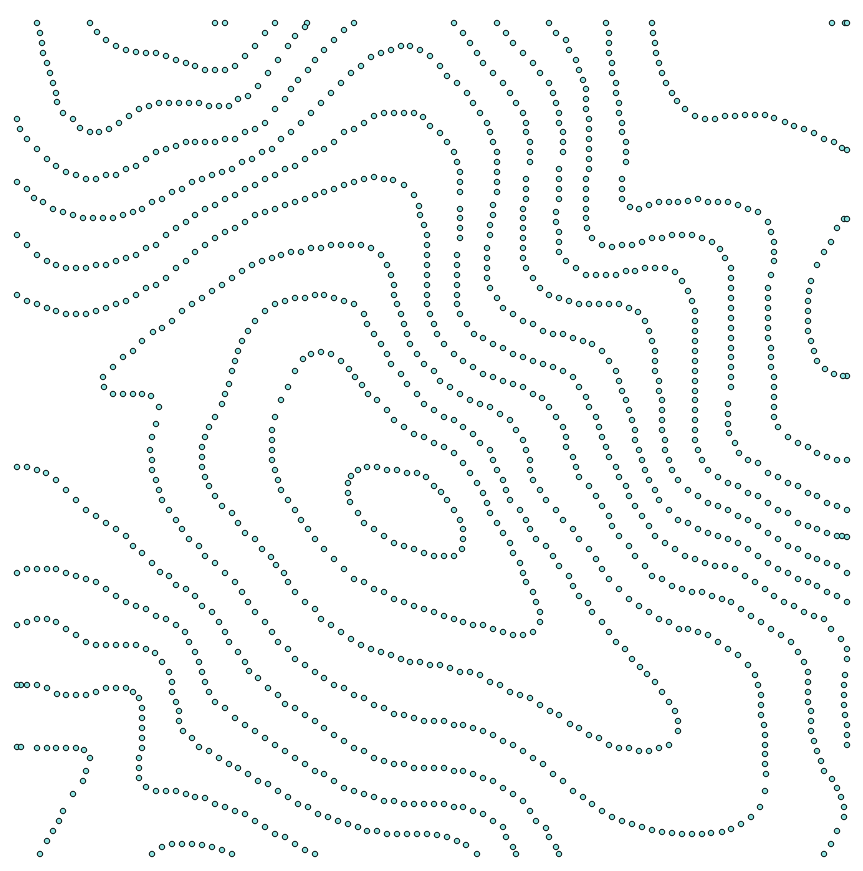
\includegraphics[width=\textwidth]{figs/wedding0.png}
    \caption{}
  \end{subfigure}%
  \begin{subfigure}[b]{0.38\linewidth}
    \centering
    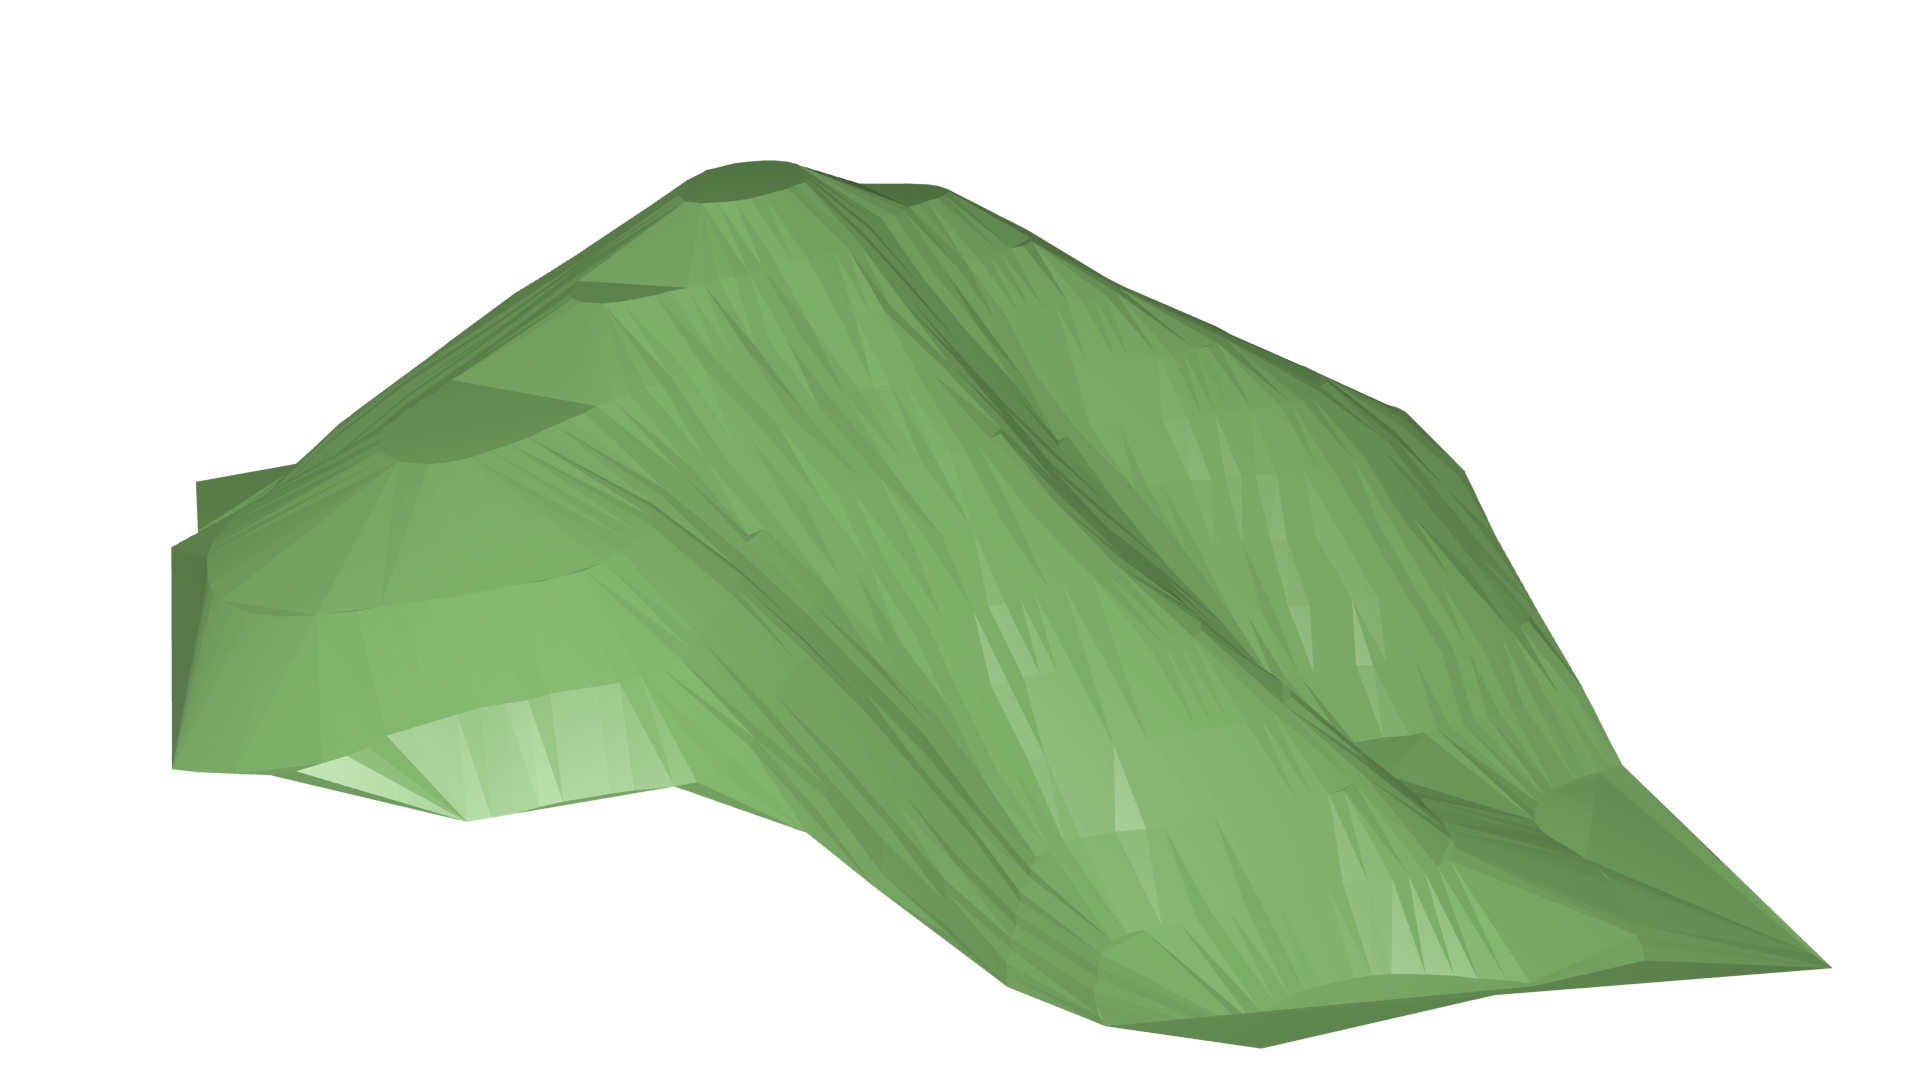
\includegraphics[width=\textwidth]{figs/wedding-tin.png}
    \caption{}
  \end{subfigure}
  \begin{subfigure}[b]{0.38\linewidth}
    \centering
    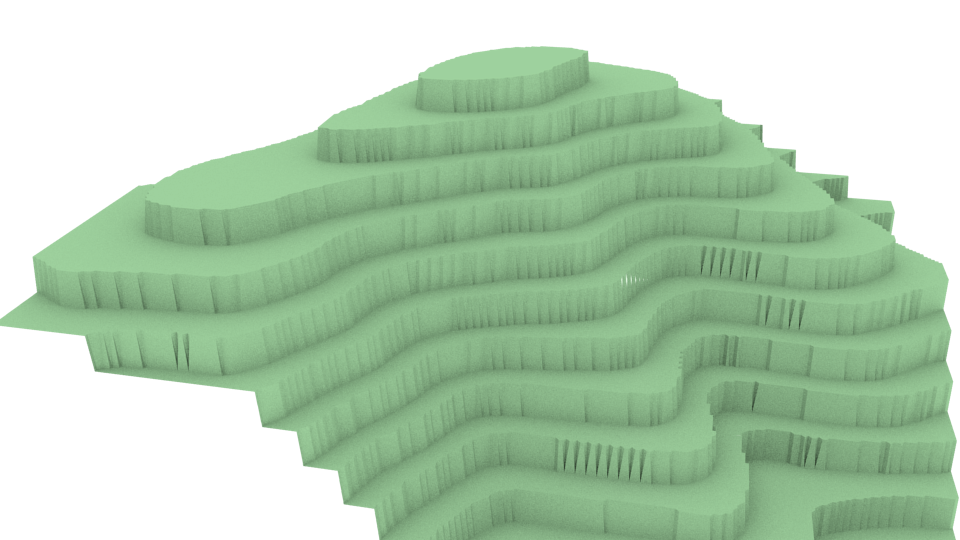
\includegraphics[width=\textwidth]{figs/wedding-nn.png}
    \caption{}
  \end{subfigure}  
\caption{The `wedding cake' effect. \textbf{(a)} The input isolines have been discretised into sample points. \textbf{(b)} The TIN of the samples creates several horizontal triangles. \textbf{(c)} The surface obtained with nearest-neighbour interpolation.}%
\label{fig:wedding}
\end{figure}
However, one should be aware that doing so will create terrains having the so-called \emph{wedding cake effect}.
Indeed, the TIN obtained with a Delaunay triangulation, as shown in Figure~\ref{fig:wedding}b, contains several horizontal triangles; these triangles are formed by 3 vertices from the same isoline.
If another interpolation method is used, \eg\ nearest neighbour (Figure~\ref{fig:wedding}c), then the results are catastrophic.

%

Solving this problem requires solutions specifically designed for such inputs.
The main ideas for most of them is to add extra vertices between the isolines, to avoid having horizontal triangles. 
One strategy that has proven to work is to add the new vertices on the \emph{skeleton}, or medial-axis transform, of the isolines, which are located `halfway' between two isolines.
The elevation assigned to these is based on the elevations of the isolines.
%\refchap{chap:mat} explains in details what the medial-axis transform is.


%%%%%%%%%%%%%%%%%%%%
%
\section{Notes \& comments}

The \emph{Implicit Function Theorem} is further explained in \citet{Sibson97}.

\citet{Dakowicz03} describe in details the skeleton-based algorithm to interpolate from isolines, and show the results of using different interpolation methods.

The basic algorithm to extract isolines, which is a brute-force approach, can be slow if for instance only a few isolines are extracted from a very large datasets: all the $n$ triangles/cells are visited, and most will not have any intersections.
To avoid this, \citet{vanKreveld96} build an auxiliary data structure, the \emph{interval tree}, which allows us to find quickly which triangles will intersect a given elevation.
It is also possible to build another auxiliary structure, the contour tree, where the triangle seeds are stored~\citep{vanKreveld97-1}.
Such methods require more storage, but can be useful for interactive environment where the user extracts isolines interactively.

\citet{Garland95} elaborate further on different aspects of TIN simplification, such as different importance measures, the differences between refinement and decimation, and the usefulness of data-dependent triangulations. 
They also show how Algorithm~\ref{algo:tin-simp:ref} can be made a lot faster by only recomputing the importance of points in triangles that have been modified. 


%%%%%%%%%%%%%%%%%%%%
%
\section{Exercises}

\begin{enumerate}
  \item When converting isolines to a TIN, what main ``problem'' should you be aware of? Describe \emph{in details} one algorithm to convert isolines (given for instance in a \emph{shapefile}) to a TIN and avoid this problem.
  \item How would the isocontours of a 2.75D terrain look like?
  \item In Section~\ref{sec:structuring}, it is mentioned that merging the segments will form on polygon. But how to ensure that the orientation of that resulting curve is consistent, that it is for instance having higher terrains on the right?
  \item Given a raster terrain (GeoTiff format) that contains several cells with \texttt{no\_data} values, describe the methodology you would use to extract contour lines from it. As a reminder, contours lines should be closed curves, except at the boundary of the dataset.
  \item Assume you have the small terrain formed of 3 triangles below, draw the isoline in this TIN for an elevation of 10m.
  \\ \\
  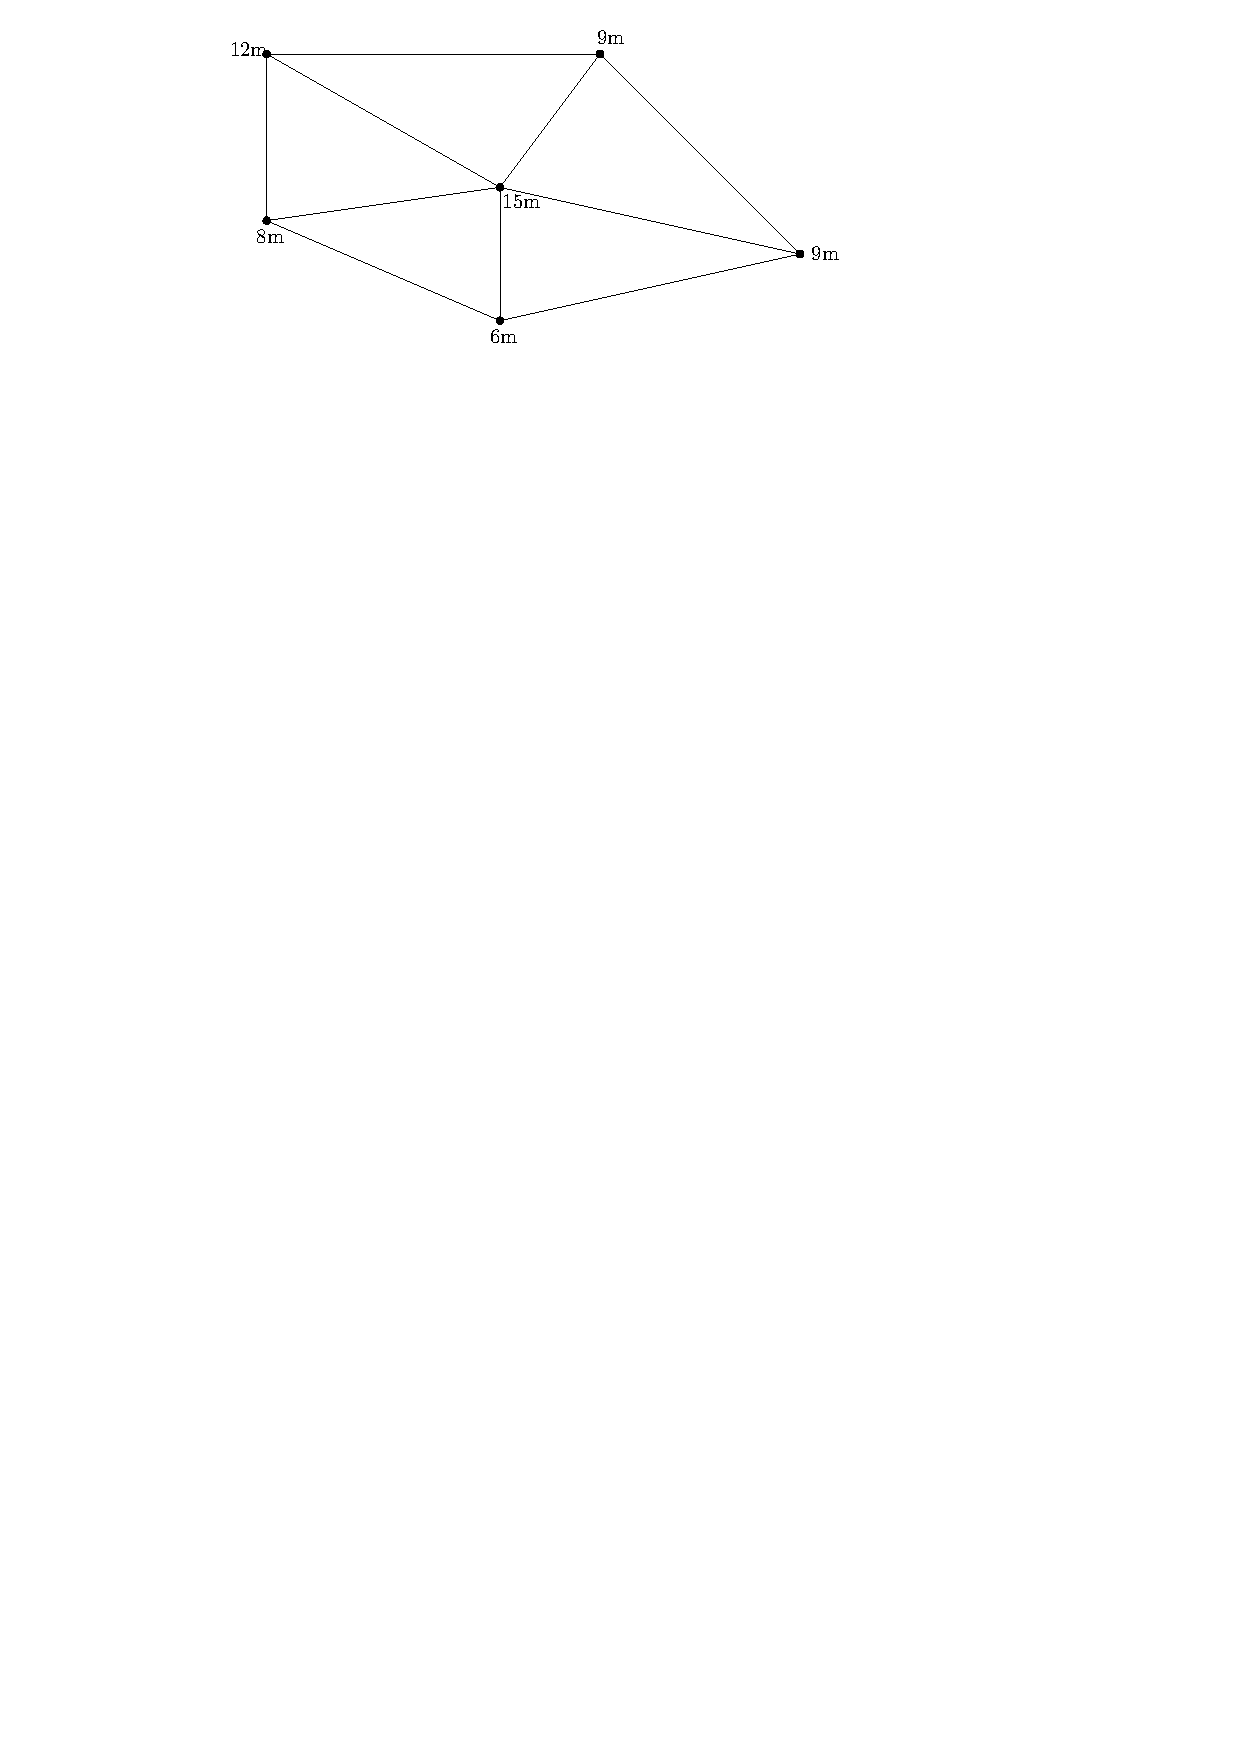
\includegraphics[width=0.5\linewidth]{figs/threetr.pdf}
\end{enumerate}